\part{Felhasználói dokumentáció}
A programcsomagot JAVA programozási nyelven írtam meg, így a program számára biztosítani kell JAVA futtatókörnyezetet, továbbá a program működéséhez adatbázis szerverre is szükség lesz. A telepítés magába foglalja az adatbázis séma elkészítését és az adatbázist demó adatokkal tölti fel, így a telepítést követően extra dolgokra nem lesz szükség.

\section{Telepítés}
\subsection{Java SE Runtime Environment 8}
A programcsomag futtatásához legalább Windows XP operációs rendszer szükséges, amelyen Java SE Runtime Environment 8 futtató környezet \cite{jresite} (a továbbiakban: JRE) fut. A JRE feltelepítését követően manuálisan ellenőrizzük, hogy a rendszer felvette-e környezeti változóként az installációs könyvtárat. Navigáljunk az operációs rendszerben a környezeti változók módosítása panelhez, majd ellenőrizzük le, hogy a PATH nevű környezeti változóhoz hozzá lett-e adva az installációs könyvtár: \path{C:\Program Files\Java\jdk1.8.0_60\bin}. 
Ha nem, akkor pontosvesszővel (;) elválasztva egészítsük ki a változó értékét, majd indítsuk el a promptot (ha nyitva van, akkor indítsuk újra).
Ha a
\begin{verbatim}
java -version
\end{verbatim}
utasítás hatására az 
\begin{figure}[h!]
  \caption{JRE verzió}
  \label{fig:jre_version}
  \centering
    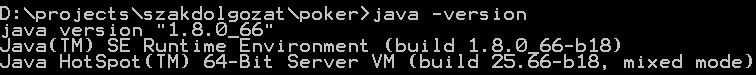
\includegraphics{user-documentation/images/java_version.jpg}
\end{figure}
 \ref{fig:jre_version}. ábrán látható szöveg jelenik meg a konzolon, akkor sikeres volt a JRE telepítése és beállítása. További instrukciókért ld. melléklet.
 
 \subsection{MySQL Community Server 5.6}
 A programcsomag megköveteli a MySQL Community Server 5.6 adatbázis-kezelő rendszer \cite{mysqlsite} (a továbbiakban: MySQL Server) használatát is. Letöltés után csomagoljuk ki a zip állományt egy tetszőleges könyvtárba, majd a fentiekkel megegyező módon adjuk hozzá a PATH nevű környezeti változó értékéhez a MySQL Server bin könyvtár elérési útvonalát. Ha ezzel végeztünk, akkor nyissük meg a promptot (ha nyitva van, akkor indítsuk újra), majd navigáljunk a MySQL Server bin könyvtárába, ott pedig adjuk ki a
 \begin{verbatim}
mysqld --install
\end{verbatim}
parancsot. A parancs végrehajtása után navigáljunk a szolgáltatások panelhez, amelyet a legkönnyebben a promptban a
 \begin{verbatim}
services.msc
\end{verbatim}
\begin{figure}[h!]
  \caption{MySQL Service}
  \label{fig:mysql_service}
  \centering
    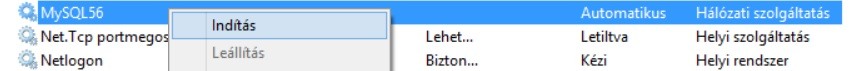
\includegraphics{user-documentation/images/mysql_service.jpg}
\end{figure}
kiadott utasítással lehet elérni. Majd járjunk el a \ref{fig:mysql_service}. ábrának megfelelően. Térjünk vissza a konzolra, ahol adjuk ki a 
 \begin{verbatim}
mysql -u root -p
\end{verbatim}
parancsot, amely jelszót fog kérni. A beviteli sort hagyjuk üresen, nyomjunk entert. Ha sikeresen beléptünk az adatbázis-kezelő rendszerbe, akkor adjuk ki a
 \begin{verbatim}
SELECT VERSION();
\end{verbatim}
utasítást, és ha a 
\begin{figure}[h!]
  \caption{MySQL Service}
  \label{fig:mysql_service}
  \centering
    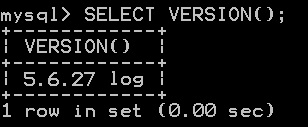
\includegraphics{user-documentation/images/mysql_version.jpg}
\end{figure}
\ref{fig:mysql_service}. ábrának megfelelő képernyőképet kapunk, akkor sikeresen feltelepítettük az adatbázis-kezelő rendszert.

\subsection{Az adatbázis használatba vétele}
Ha sikeresen elindítottuk a MySQL Servert, akkor szükségünk lesz egy új adatbázis sémára (és demo adatokra), amelyet a \path{X:\poker\release\poker-db.sql} állományban találunk. Ezt a filet kell lefuttatni az adatbázison, a hatása idempotens. A promptban adjuk ki a
 \begin{verbatim}
mysql -u root -p < X:\poker\release\poker-db.sql
\end{verbatim}
utasítást, amely jelszót fog kérni. A beviteli sort ugyancsak hagyjuk üresen. Ha sikeresen lefutott a parancs, akkor az adatbázis séma ``felhúzása'' megtörtént.

\section{A póker játékról}
A póker, mint kártyajáték igen népszerű szerencsejáték. Akár élő tv adásokat is végig lehet követni, ahol hatalmas főnyereményeket osztanak ki a dobogós helyezetteknek. Viszonylag sok fajtája terjedt el szerte a világon, kezdve a klasszikus 5 lapos leosztásokkal egészen az OMAHA-án át a jól ismert Texas Hold'Em játékstílusig. A játékot 52 lapos francia kártyapaklival játszák, amelyben 4 szín és 13 különböző értékű kártyalap található. A játékcélja, hogy minél több zsetont gyűjtsünk össze a partik során.

\section{Fogalomtár}

\subsection{Játékmenet}
Minden játékszerver úgy lett konfigurálva, hogy két játékos esetén a parti elkezdődjön. Ha valaki később csatlakozott az asztalhoz, az a megkezdett partiból semmit nem érzékel, mintha üres asztalnál ülne. Csak a következő partiba tud beszállni. Mindkét játékstílus esetén van egy BLIND kör, amikor a szerver bekéri a vakokat a játékosoktól. Az osztótól eggyel balra ülő játékos köteles betenni a kis vakot, a kis vaktól eggyel balra ülő játékos pedig köteles betenni a nagy vakot. Ebból a felhasználó nem lát semmit, köteles beadni a kis- vagy nagyvakot, amelyet egy automatizált eljárás hajt végre. Az osztó gomb  a legelső körben kerül kiosztásra a legelsőként csatlakozott játékoshoz. Az osztó gomb az óramutató járásával megegyező irányban halad. Minden új megkezdett parti esetén az osztó gomb a következő játékoshoz kerül. Minden parti legelső körében a kezdő játékos az osztótól balra ülő harmadik játékos, minden további kört a kis vakra kötelezett játékos kezd meg.  \\
A játékszerverek nem képesek kezelni, ha egy játékosnak elfogyott, illetve nincs elegendő zsetonja. Ebből kifolyólag esetenként előfordulhat negatív egyenleg, illetve nem definiált viselkedés. A játékosok szigorúan csak egymást követve küldhetnek utasításokat a szervernek, mindig az éppen soron levő játékos. A felhasználói grafikus felületen egyértelmű jelzéssel van ellátva az éppen soron levő játékos. A játékosok megadhatják (CALL), emelhetik (RAISE) a tétet, illetve, ha nem szeretnének az adott körben semmit csinálni, akkor CHECK-elhetnek. Az emelés mértéke a mindenkori játékasztal alaptét felét jelenti. Ugyanakkor lap eldobásra (FOLD) és a játék elhagyására (QUIT) is lehetőség van. A felhasználók (korlátozottan) visszanézhetik a korábbi leosztásokat, és a partiban történt eseményeket (LOG). A játékosok asztalonkénti maximum száma 5 fő. A kliensek a játék elhagyását követően újracsatlakozhatnak az adott játékszerverre a fentieket figyelembe véve. Lehetőség van asztalt váltani, és a játékszerverek (korlátozottan) képesek kezelni, ha a játékossal megszakad a kapcsolat. A kliens alkalmazások is (korlátozott mértékben) fel vannak készítve az esetleg kommunikációs hibákra.

\subsection{Játékstílusok} \label{subsubsec:game_styles}
A program kettő beépített játékstílust definiál
\begin{itemize}[leftmargin=2cm]
\item Classic \cite{five_card_draw}
\item Texas Hold'Em \cite{texas_holdem}
\end{itemize}

\pokerparagraph{Classic} 
A klasszikus játékstílus legfőbb ismertető jele, hogy mindenki öt lapot kap kézbe és nincsenek közös lapok. Először is a vakokra kötelezett játékosok rakják be a vakokat (automatizáltan), azután pedig úgynevezett pre-round van, amikor a szerver minden játékosnak öt-öt lapot oszott kézbe, és ezek alapján lehet licitálni. Ha vége a körnek, akkor mindenki kicserélheti a lapjait, amiket saját maga választ ki a grafikus felületen a saját kártyalapjainak rákattintásával. Ha a kártyalap ``feljebb'' csúszott a grafikus megjelenítésen, akkor a kártyalapot cserére jelölte a játékos. A CHANGE feliratú gombbal cserélhetőek a kártyák. Mindenki akkor kapja meg az új kártyalapjait, ha már mindenki nyilatkozott a cseréről. Ezek után új kör indul, amikor is az új lapok birtokában tehetik meg a tétjeiket a játékosok. A kör után a szerver kihirdeti a nyertest, és a nyertes lapokat az asztal közepén jeleníti meg a grafikus felület. Kivétel, ha a nyertesek az éppen adott felhasználó, akkor a nyertes kártyalapok maga előtt jelen vannak, más kártyalapok nem kerülnek felfordításra. A felhasználók a nyertes lapok megtekintését követően kötelesek rákattintani a CHECK feliratú gombra (vagy majd megcsinálom, hogy automatizált quit legyen ez is.... csak most még bugos.... winnercardsnál úgy is van nullpointerexceptionöm....). Ha ebben a körben is mindenki nyilatkozott, akkor a játékasztal új partit indít.

\pokerparagraph{Texas Hold'Em}
A klasszikus játékstílussal erősen megegyező játékmenetű stílus. A különbség csupán annyi, hogy a ház 2-2 lapot oszt minden játékosnak, amelyekkel a játékosok a parti végéig rendelkeznek. Illetőleg a nyertes lapok semmilyen esetben sem középen, hanem a játékosoknál jelennek meg.

\section{Futtatás}

\subsection{A póker szerver elindítása}
A DVD lemezen a \path{\poker\release\} mappában található meg a poker-server-1.0.0.jar file. Nyissunk egy terminált a kijelölt könyvtárban, és adjuk ki a
 \begin{verbatim}
java -jar poker-server-1.0.0.jar
\end{verbatim}
parancsot. 
\begin{figure}[h!]
  \caption{Szerver}
  \label{fig:server_started}
  \centering
    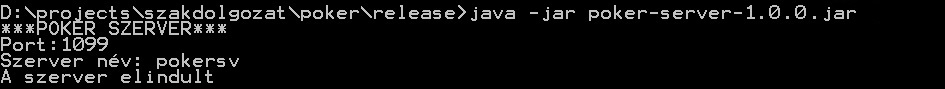
\includegraphics{user-documentation/images/server_started.jpg}
\end{figure}
Ha a \ref{fig:server_started}. ábrának megfelelő konzol loglistát látunk, akkor a szervert sikeresen elindítottuk.

\subsection{A póker kliens elindítása}
A kliens futtatása hasonló módon történik, mint a szerveré. Navigáljunk a \path{\release\poker\kliens} mappába, és a konzolon adjuk ki a megfeleő parancsot.
Jöhet az ábra, meg a kódot kicsit átírni, hogy logoljon konzolra, mint a szerver...

\section{A póker játék használata} %Csatlakozás a játékhoz
\begin{figure}[h!]
  \caption{Bejelentkezési form}
  \label{fig:client_login}
  \centering
    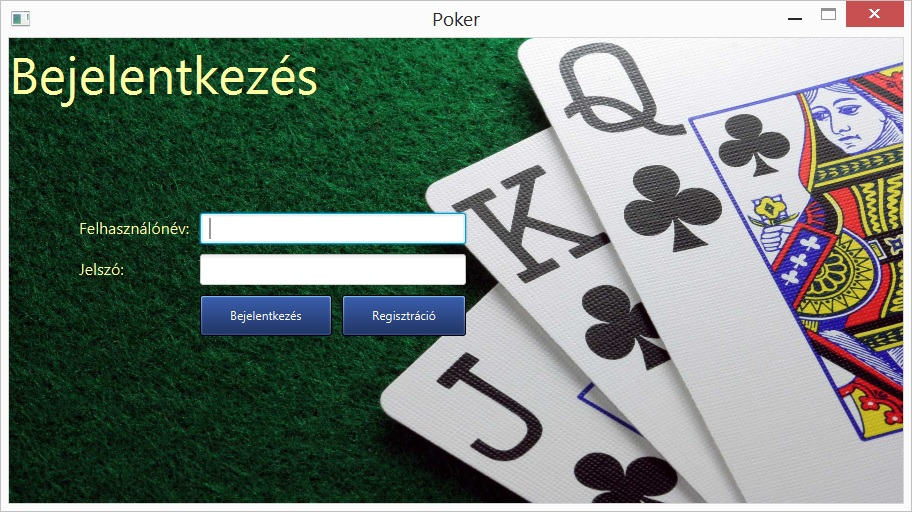
\includegraphics[width=\textwidth]{user-documentation/images/login.jpg}
\end{figure}
A játék indítása után az \ref{fig:client_login}. ábrán látható bejelentkező felületet kapjuk. Ha még nem regisztráltuk magunkat a játékba, akkor kattinstunk a Regisztráció nevű gombra, amely felület a X. ábrán szerepel. Adjuk meg a regisztrálni kívánt felhasználó nevünket és jelszavunkat, majd regisztráljunk.  (Képek kellenek ide, error, info?) A szerver értesít minket, hogy a művelet sikeres, vagy sikertelen volt. Ügyeljünk arra, hogy névütközéseket a szerver nem enged. Tehát, ha valaki XYZ névvel már regisztrálva van, akkor még egy ugyanolyan nevű felhasználót nem enged regisztrálni a szerver. Továbbá győződjünk meg arról, hogy a megadott jelszavak megegyeznek.  \\
Sikeres regisztrációt követően a program visszairányít minket a bejelentkezési formhoz, amelyet értelemszerűen kitöltve be tudunk jelentkezni a programba.
A sikeres bejelentkezést követően a
\begin{figure}[h!]
  \caption{Játékasztalok}
  \label{fig:poker_tables}
  \centering
    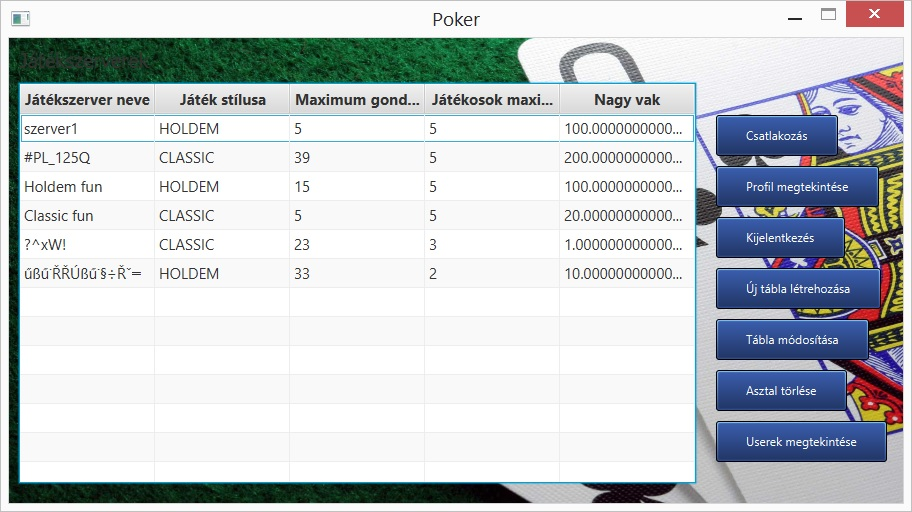
\includegraphics[width=\textwidth]{user-documentation/images/tables.jpg}
\end{figure}
\ref{fig:poker_tables}. ábrán látható felület fogad minket, ahol például asztalhoz csatlakozhatunk. Tetszőlegesen válasszunk ki egy asztalt, majd kattintsunk a Csatlakozás feliratú gombra.
\begin{figure}[h!]
  \caption{Üres játékasztal}
  \label{fig:empty_table}
  \centering
    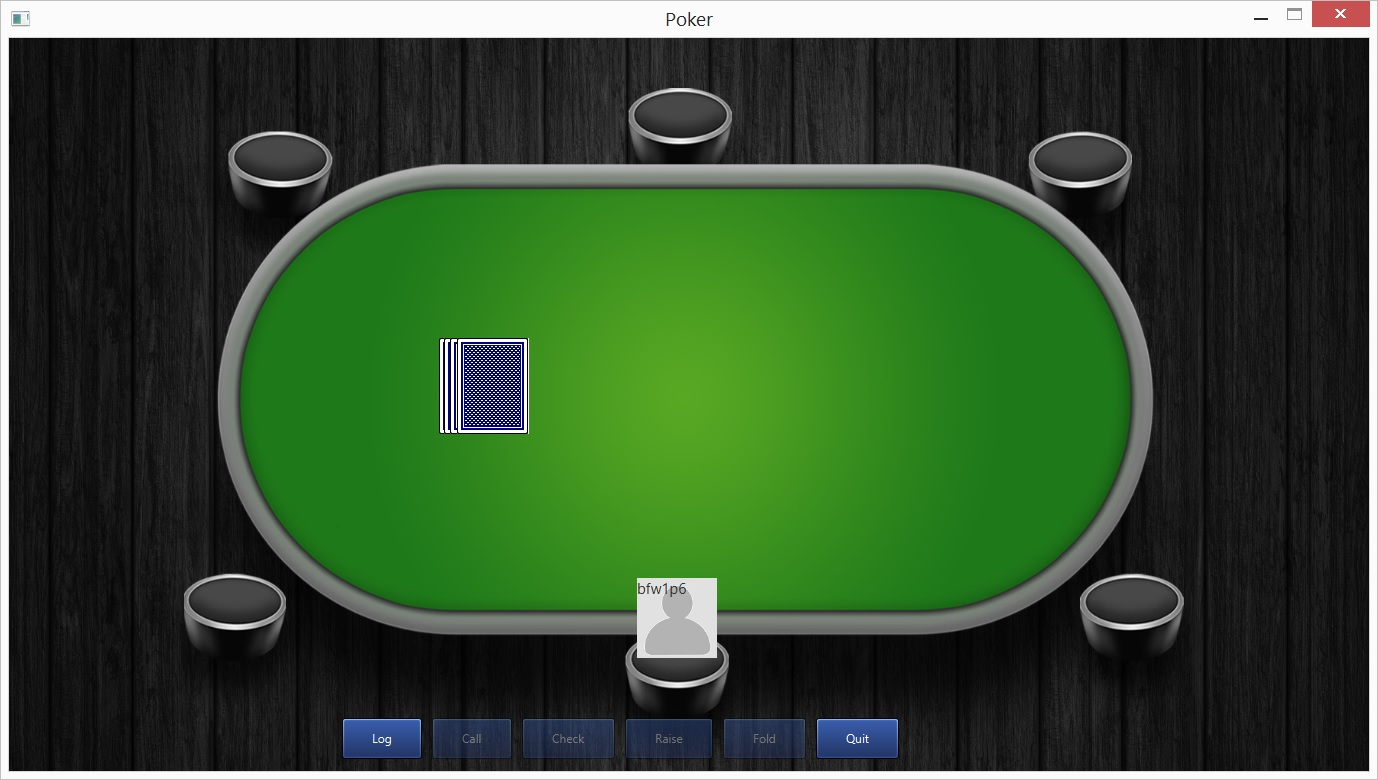
\includegraphics[width=\textwidth]{user-documentation/images/empty_table.jpg}
\end{figure}
A program átirányított minket a \ref{fig:empty_table}. ábrán jelölt felületre. Az üres játék asztal (optimális esetben) két dolgot jelenthet, vagy azt, hogy az asztalnál éppen játszanak, vagy pedig azt, hogy az asztalnál mi vagyunk az egyedüli játékosok. Indítsunk el egy második klienst (hivatkozás?) is, majd csatlakozzunk ugyanahhoz az asztalhoz, amelyiknél az előző kliens helyet foglalt. A játék (optimális esetben) elindult, és ha az asztal klasszikus játékstílusú, akkor
\begin{figure}[h!]
  \caption{Klasszikus játékstílusú asztal}
  \label{fig:classic_table}
  \centering
    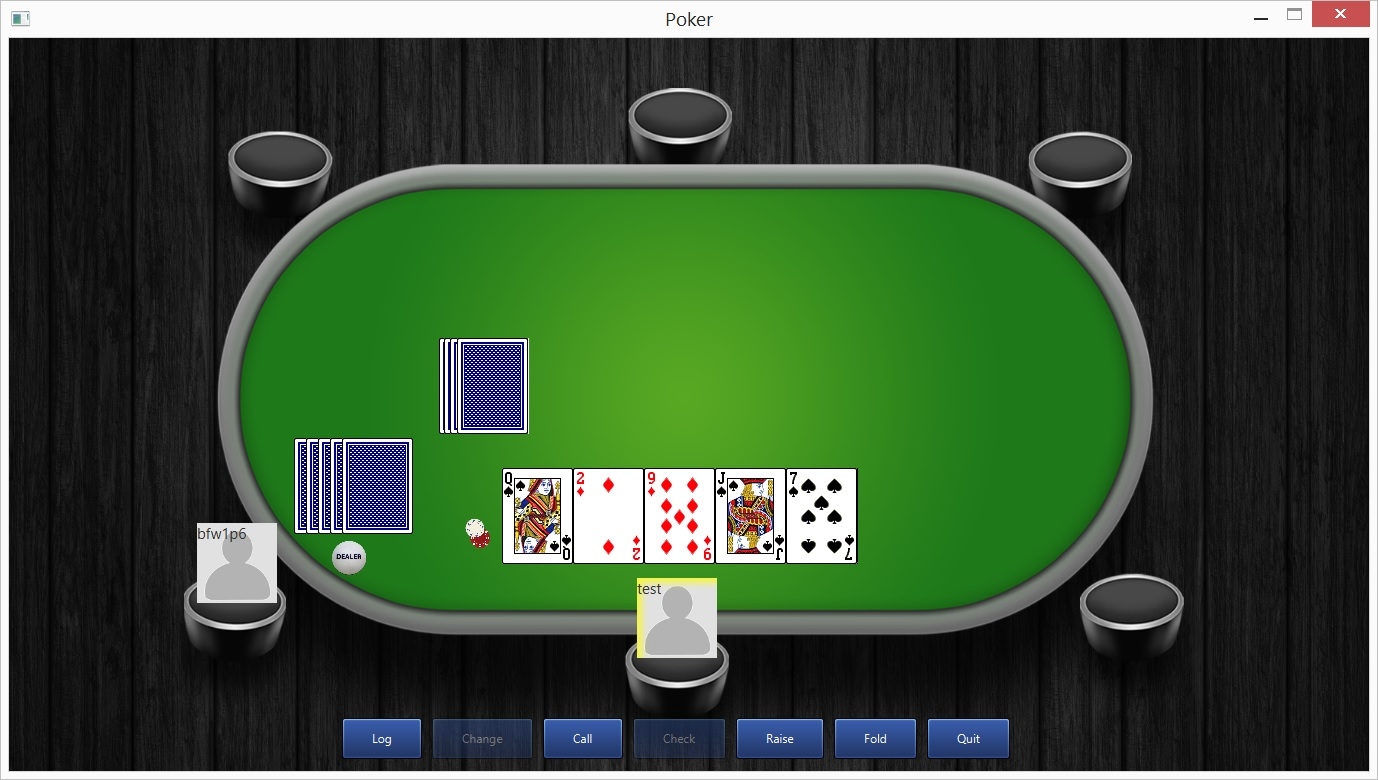
\includegraphics[width=\textwidth]{user-documentation/images/classic_game.jpg}
\end{figure}
\ref{fig:classic_table}. ábrán látható felület fogad minket.

\clearpage
